\chapter{Dataset}

This chapter describes the used datasets, presenting their construction methodology and a brief descriptive analysis.

\section{End-to-End Packet Loss Fraction Time Series Dataset}

\subsection{Methodology}

The results presented in this work are collected from cable-television infrastructure running DOCSIS with asymmetric download and upload bandwidths. The measurement infrastructure consists of regular home routers connected to the cable modem that run a software (from TGR, developed in partnership with UFRJ) to measure link throughput, round trip latency, loss rates, among others. Each home router communicates with one or more measurement servers devoted to execute the different measurement protocols and to store data. Measurement values from each home router are consolidated twice per hour and, by the end of every day, they are transferred to a database for analysis. The servers are strategically located by the ISP and, since the same home router can connect to more than one server, metrics from the same client to different servers can be contrasted. The resulted time series are unevenly due to a variate of reasons. One of them is that measurements are initiated only if the residential link is not under use by the ISP customer, another one is that the home router can be without Internet access or even eletrical energy.

The focus of this work is to analyze the loss fraction, however, \cite{a_preliminary_performance_measurement_study_of_residential_broadband_services_in_brazil} presents a further analysis on other metrics. Round trip packet loss fraction between the home router and the associated server is obtained by sending a train of short UDP packets by the home router and bounced back by the server. The interval between two packets in a train is configurable as well as the length of the train. The data presented in this work considers a train of 100 UDP packets of 32 bytes in which packets are 1 milliseconds apart.

\subsection{Descriptive Analysis}

The TGR software run in a subset of the ISP customers in several brazilian states. In the analysis of this section, was analysed the period from 01 may 2016 to 20 may 2016. Were selected every home router that measured at least one time and that all measures occurred to same server which necessaryly belonged to the same ufs. This filter resulted in 1870 clients time series and 1537272 measures.

In figure~\ref{fig:loss_fraction_cdf} is presented the packet loss CDF of all time series. It is possible to note that 93.2\% of the measures have zero losses.

\begin{figure}[H]
    \centering
    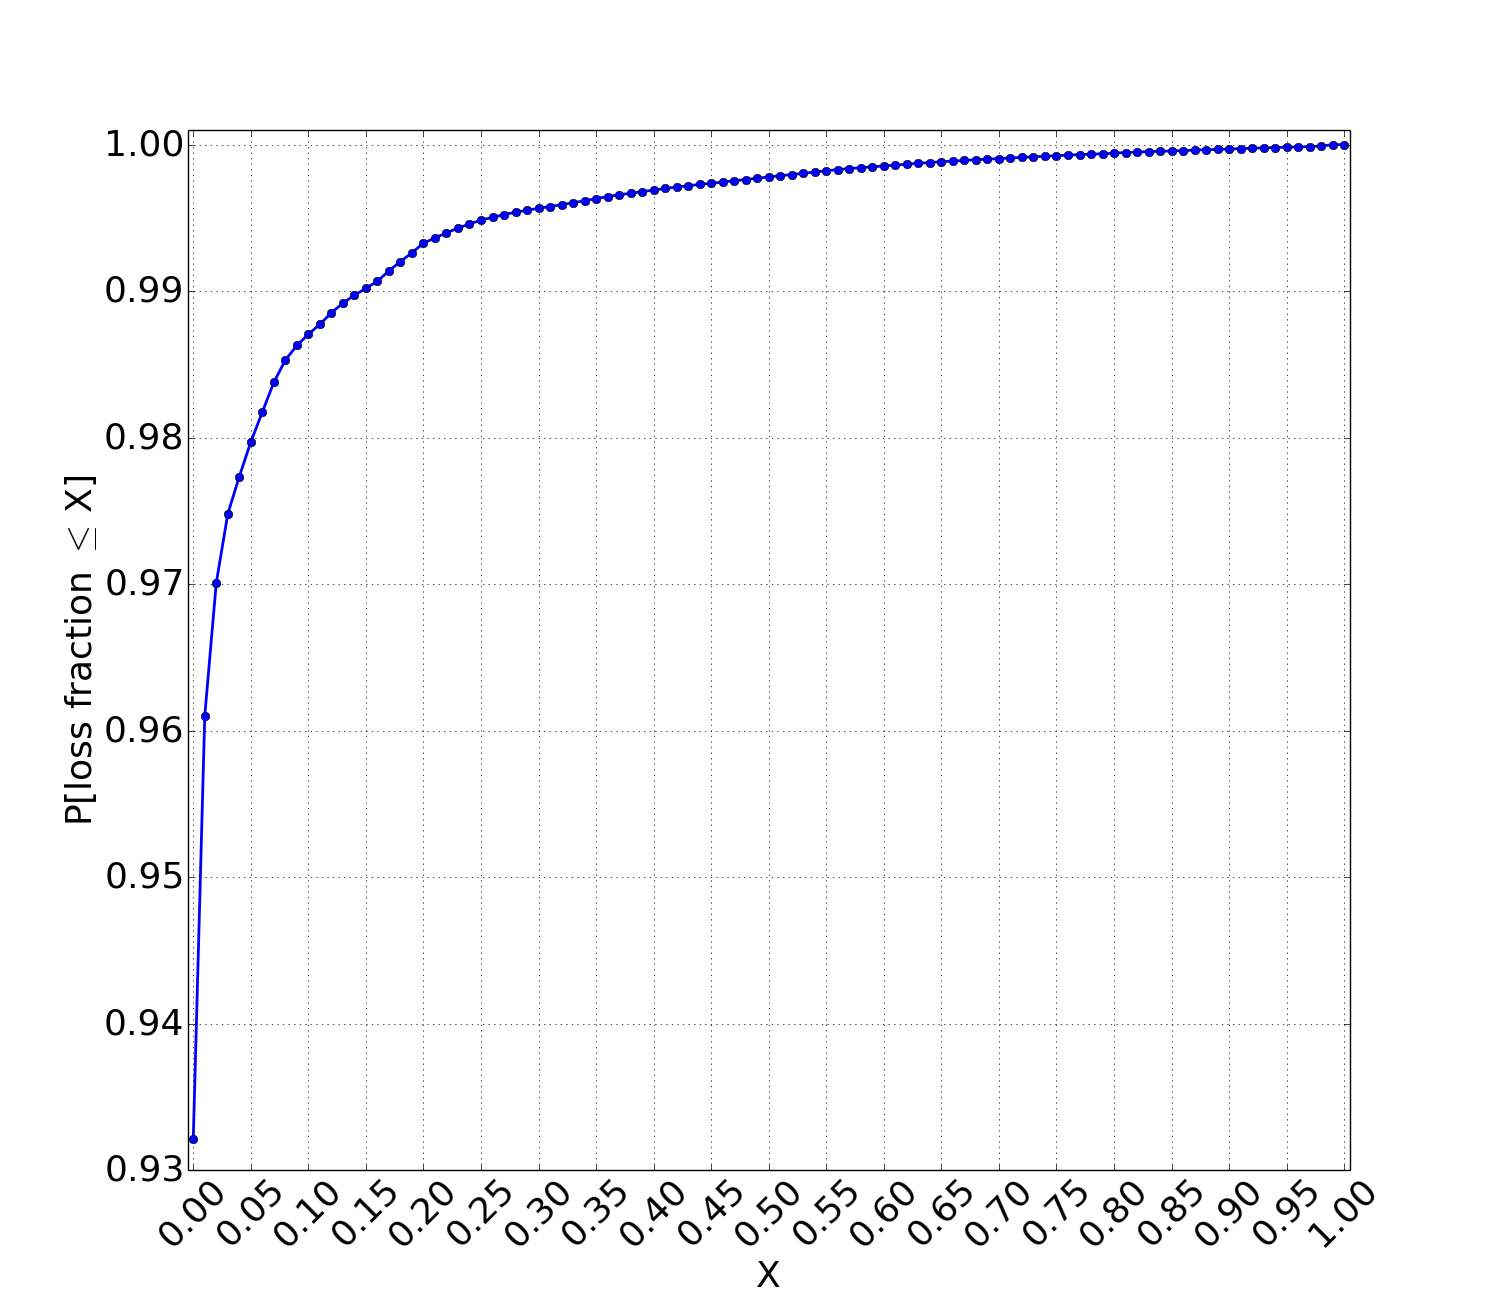
\includegraphics[width=1.0\textwidth]{./figures/loss_cdf.png}
    \caption{Packet loss fraction CDF.}
    \label{fig:loss_fraction_cdf}
\end{figure}

Figures \ref{fig:acf_ts_1}, \ref{fig:acf_ts_2}, \ref{fig:acf_ts_3} show three examples with common autocorrelation patterns in this dataset together with the time series. Since the time series are unenvely, to compute the autocorrelation function, the raw time series is transformed, and it is only considered the date and hour of a measure, ignoring the minutes and seconds. Therefore, if more than one measure occurs in the same hour, it is considered the mean.

\begin{figure}[H]
    \centering
    \begin{subfigure}[b]{0.5\textwidth}
        \centering
        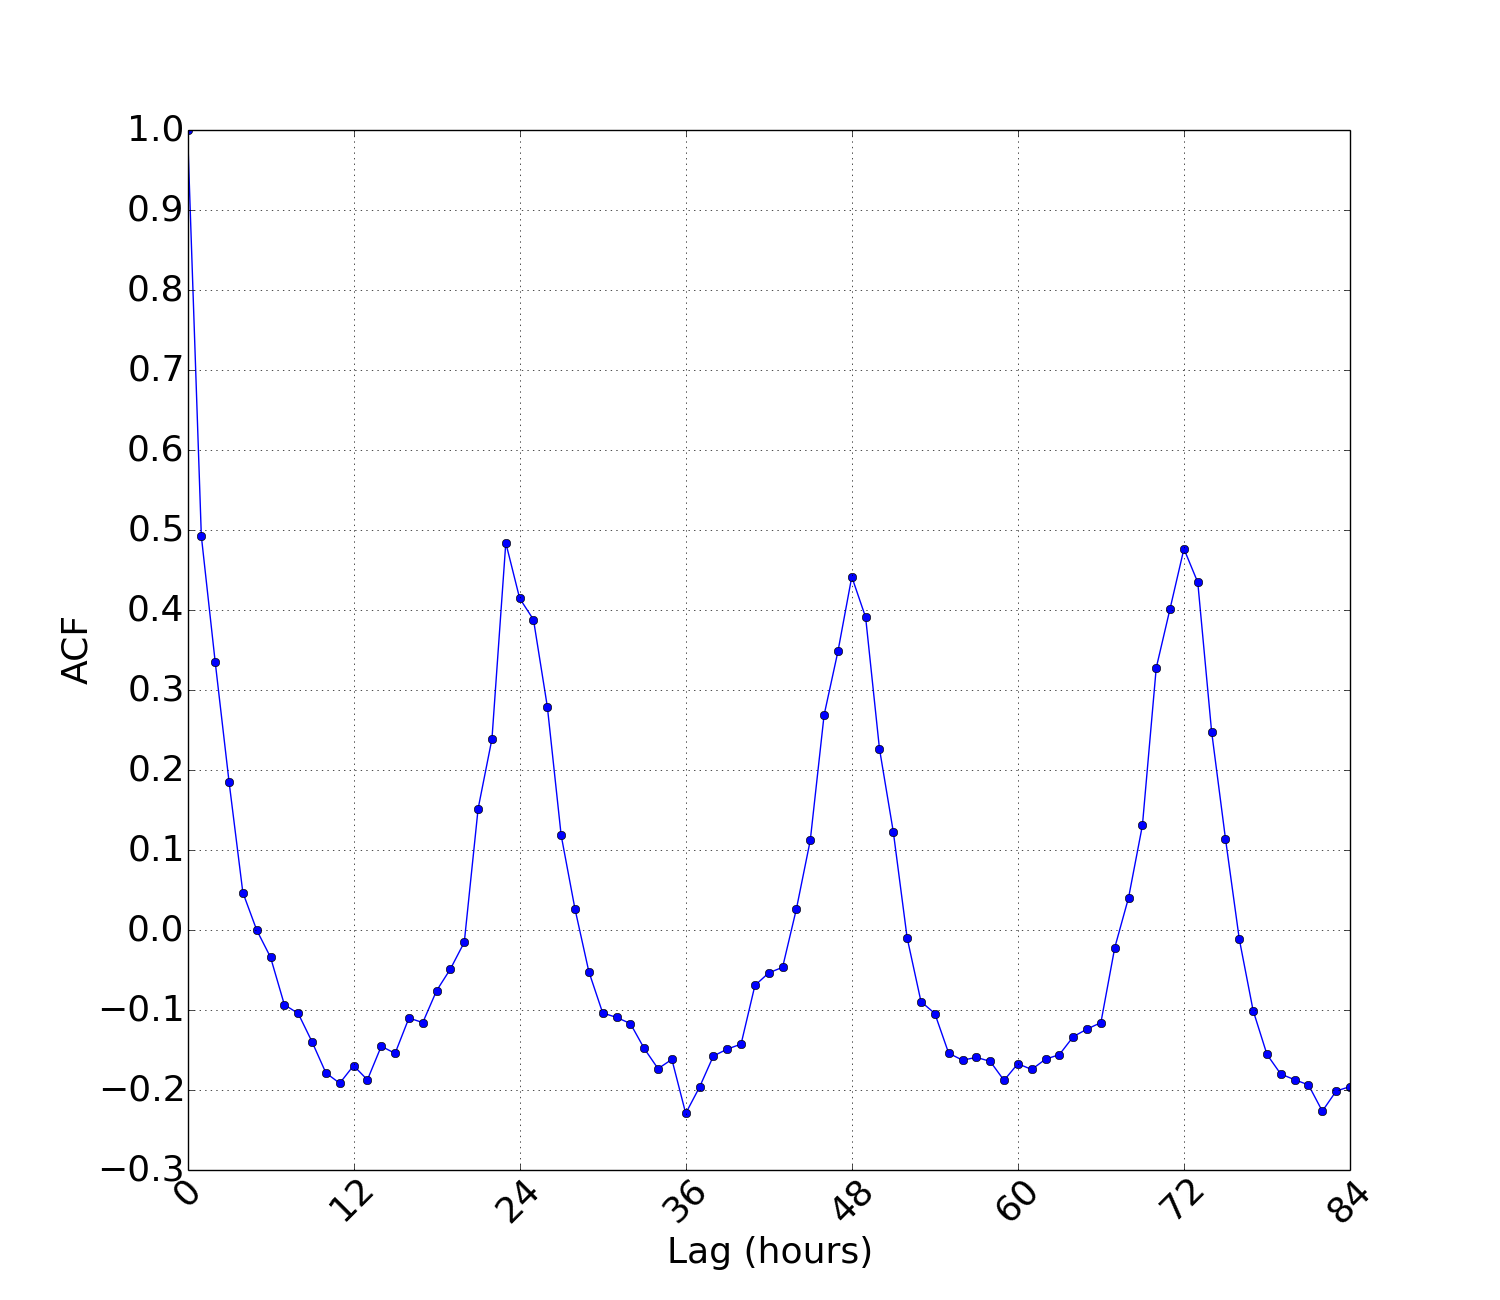
\includegraphics[width=1.0\textwidth]{./figures/acf_NHODTCSRV04_64:66:B3:50:05:BC.png}
        \caption{Autocorrelation}
    \end{subfigure}%
    ~ 
    \begin{subfigure}[b]{0.5\textwidth}
        \centering
        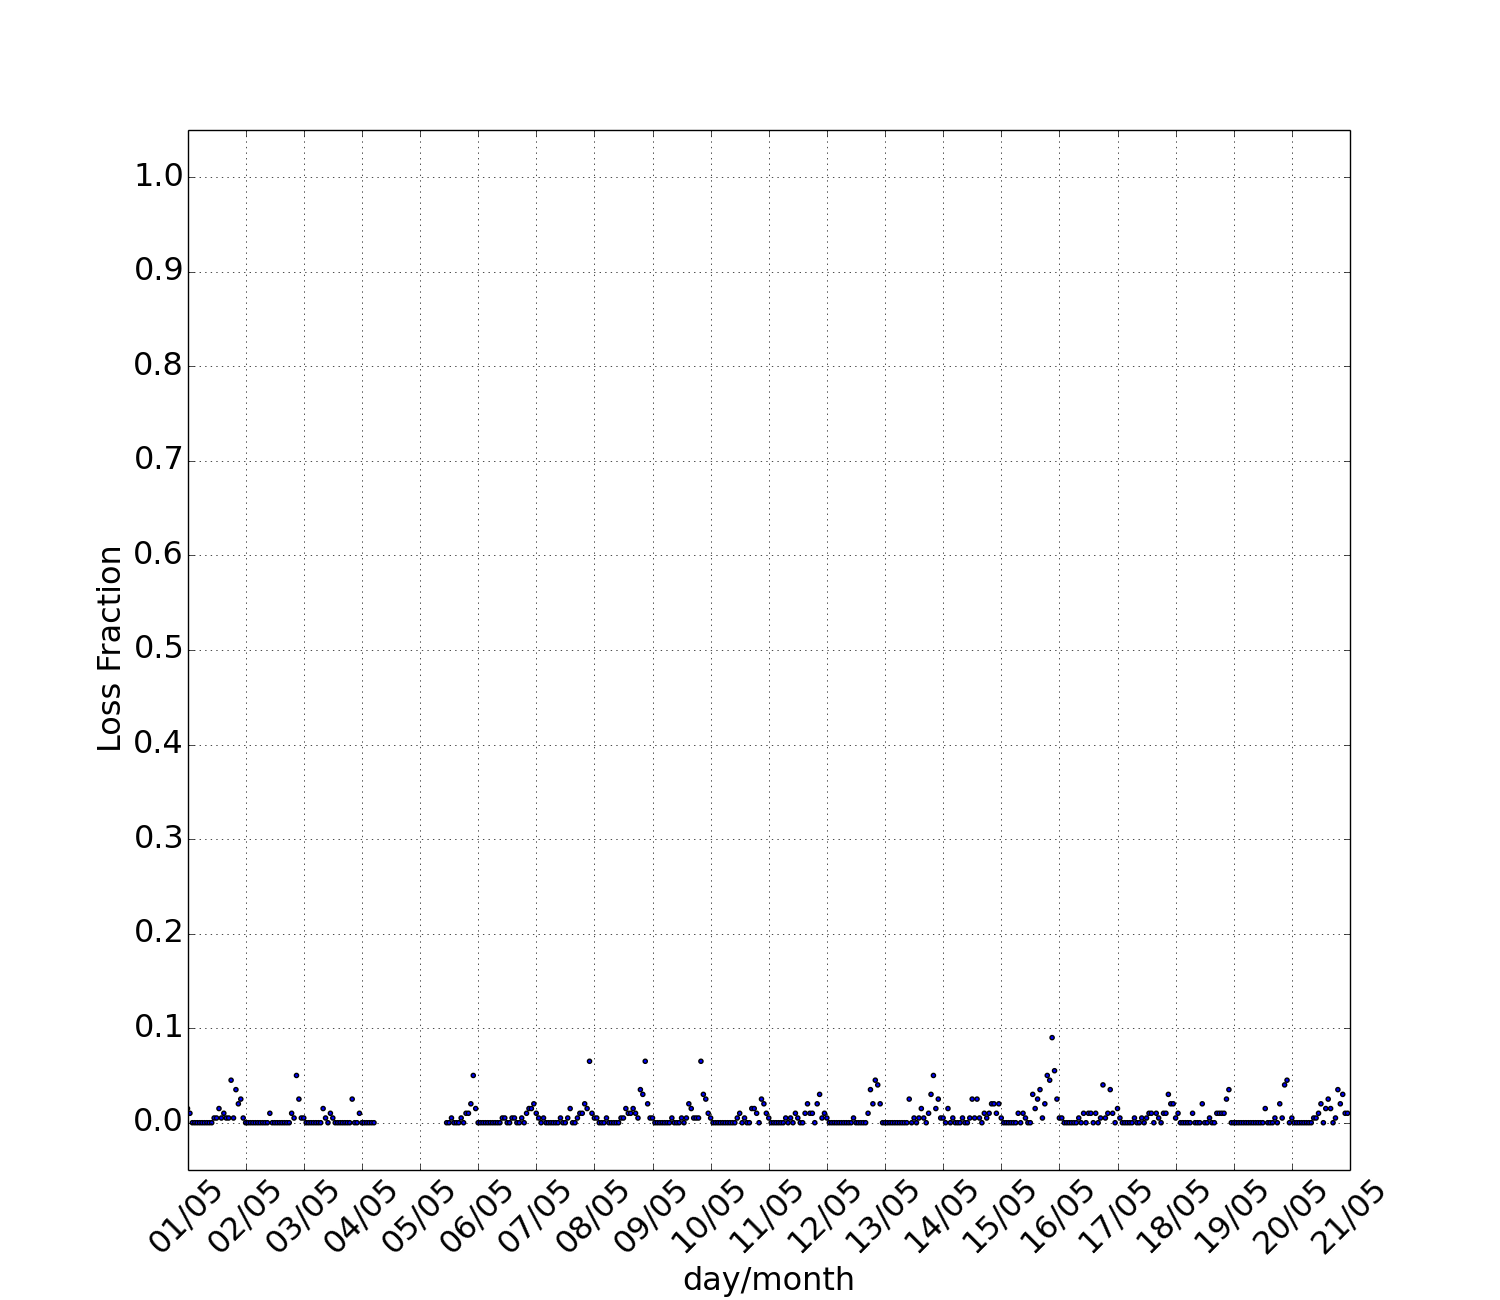
\includegraphics[width=1.0\textwidth]{./figures/ts_NHODTCSRV04_64:66:B3:50:05:BC.png}
        \caption{Time Series}
    \end{subfigure}
    \caption{Client 1}
    \label{fig:acf_ts_1}
\end{figure}

\begin{figure}[H]
    \centering
    \begin{subfigure}[b]{0.5\textwidth}
        \centering
        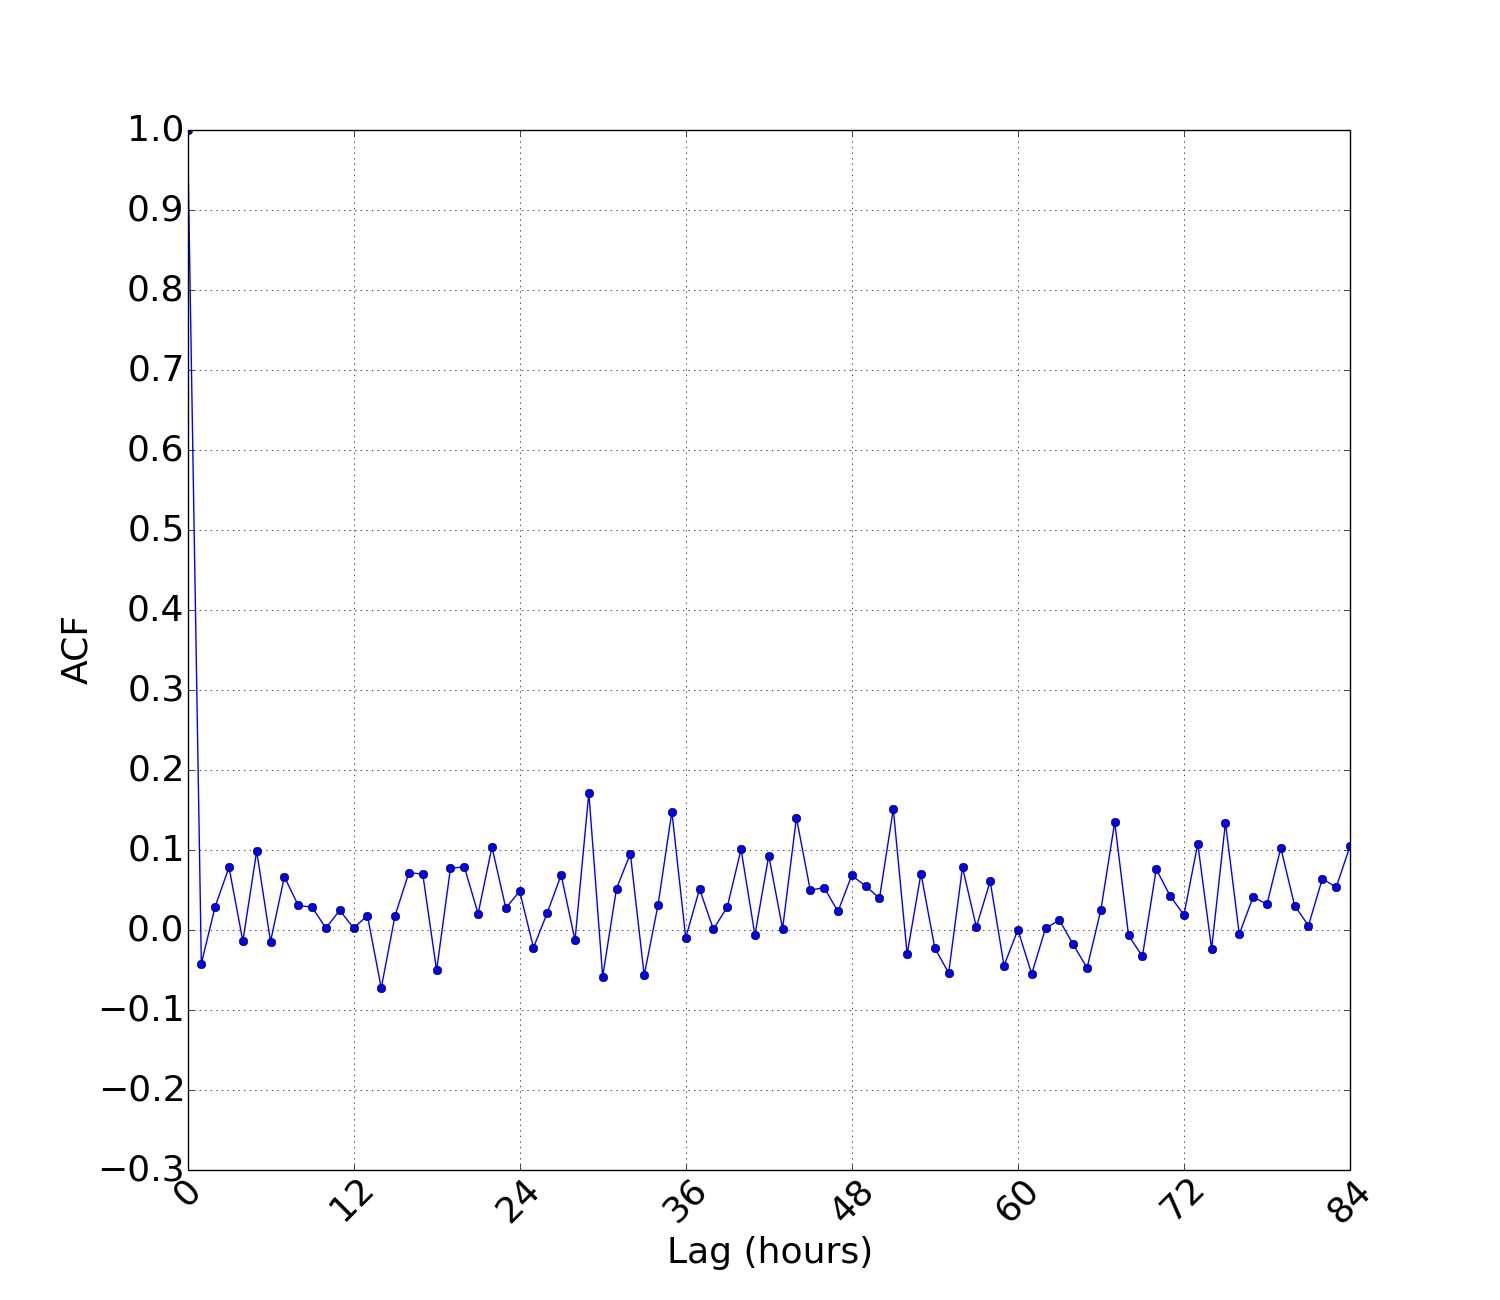
\includegraphics[width=1.0\textwidth]{./figures/acf_BREDTCSRV20_64:66:B3:7B:9E:6A.png}
        \caption{Autocorrelation}
    \end{subfigure}%
    ~ 
    \begin{subfigure}[b]{0.5\textwidth}
        \centering
        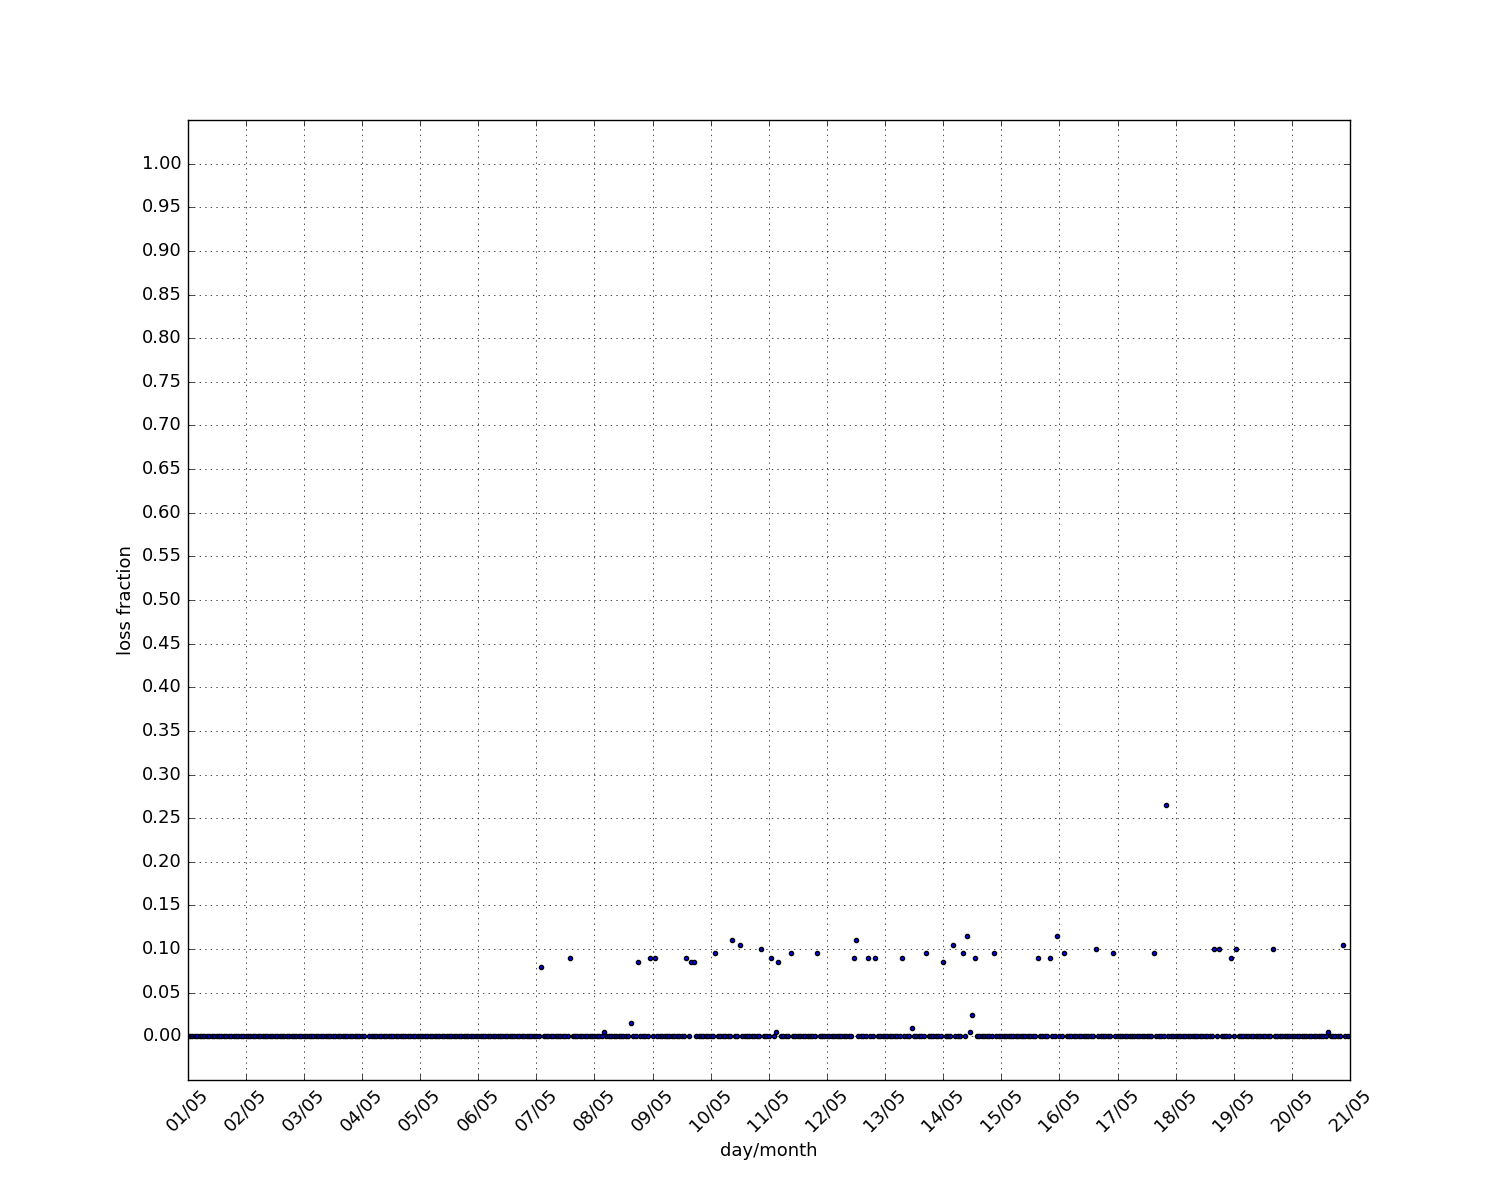
\includegraphics[width=1.0\textwidth]{./figures/ts_BREDTCSRV20_64:66:B3:7B:9E:6A.png}
        \caption{Time Series}
    \end{subfigure}
    \caption{Client 2}
    \label{fig:acf_ts_2}
\end{figure}

\begin{figure}[H]
    \centering
    \begin{subfigure}[b]{0.5\textwidth}
        \centering
        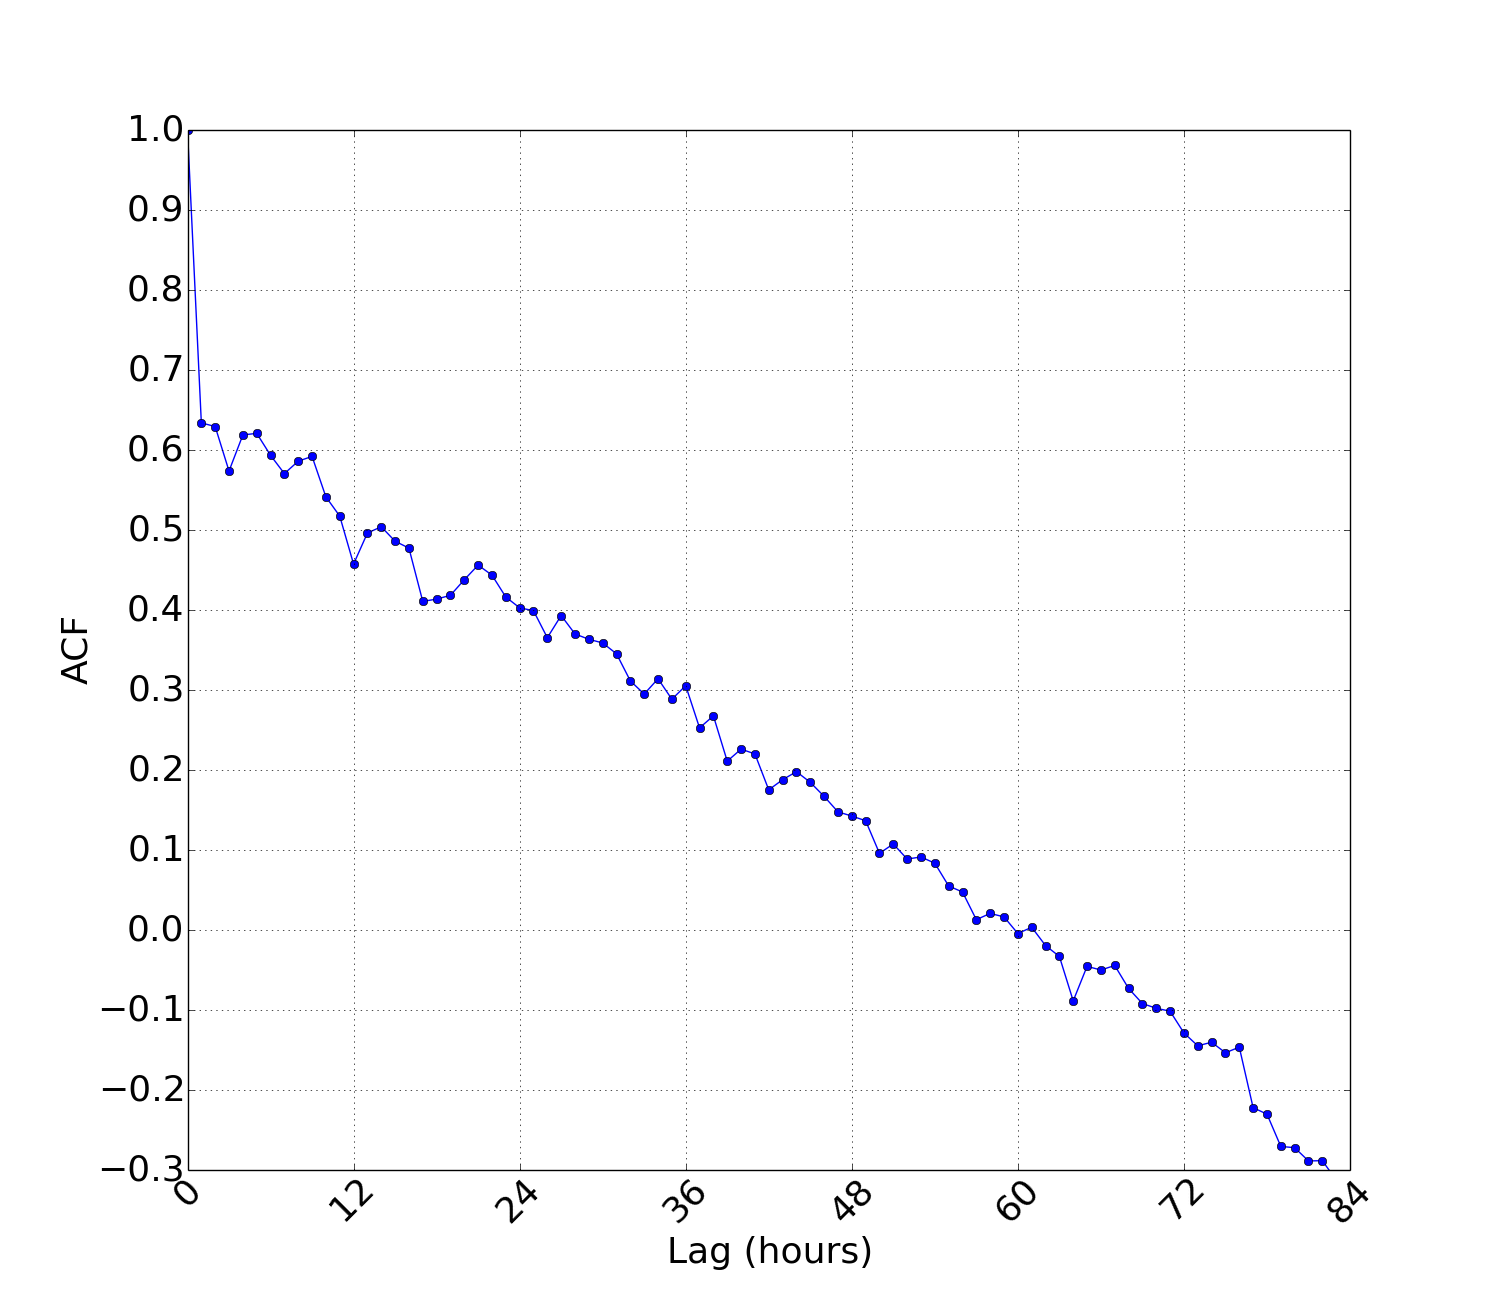
\includegraphics[width=1.0\textwidth]{./figures/acf_BHZRENPEV01_64:66:B3:A6:BA:54.png}
        \caption{Autocorrelation}
    \end{subfigure}%
    ~ 
    \begin{subfigure}[b]{0.5\textwidth}
        \centering
        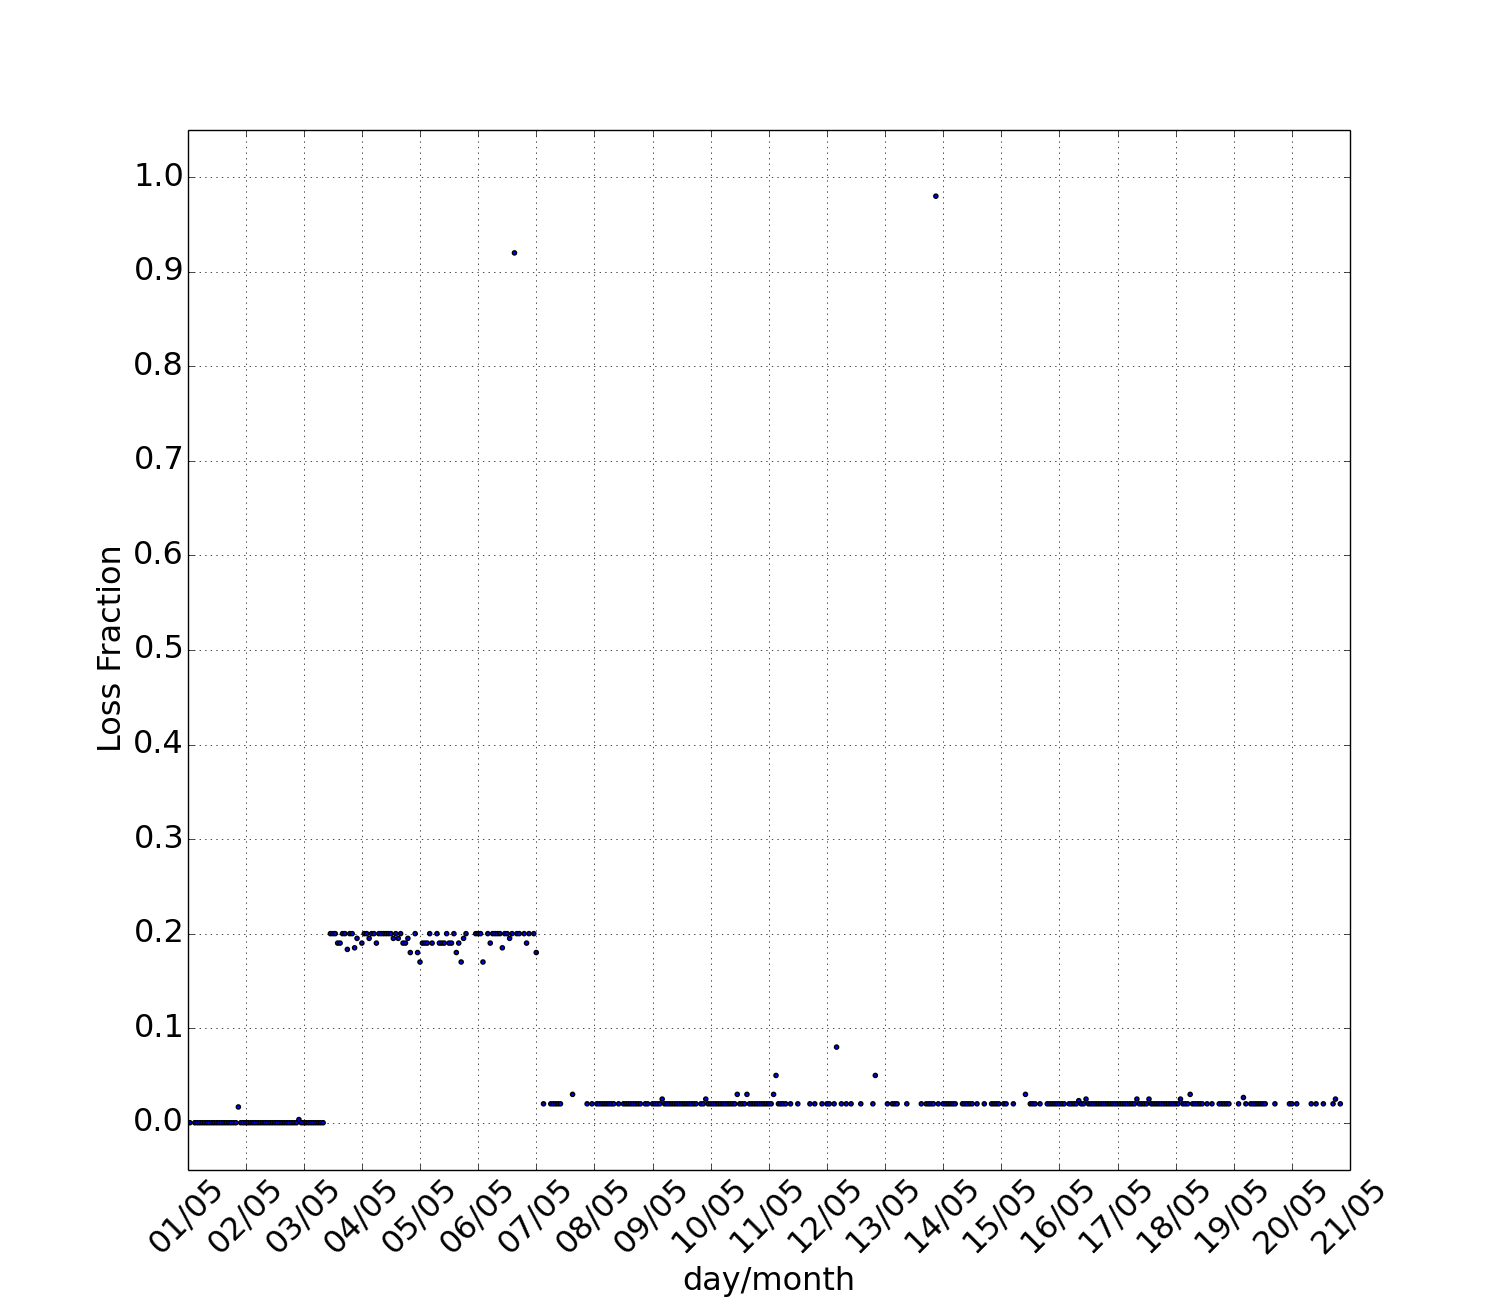
\includegraphics[width=1.0\textwidth]{./figures/ts_BHZRENPEV01_64:66:B3:A6:BA:54.png}
        \caption{Time Series}
    \end{subfigure}
    \caption{Client 3}
    \label{fig:acf_ts_3}
\end{figure}

The autocorrelation of figure~\ref{fig:acf_ts_1} have a periodic pattern, with peaks in multiple of 24 hours. In this client, it is possible to observe that losses a more frequent in the end of the day. However, in figure~\ref{fig:acf_ts_2} the autocorrelation quickly decreases and fluctuates around zero. The correspondent time series have a commmon characteristics, until day 06 of may there no measures with losses, however, from then on frequently measures with losses alternated with zero losses measures. Figure~\ref{fig:acf_ts_3} shows an linear decreasing autocorrelation, and the associated time series, which presents abrupts change in the mean. 

Also, through a visual analysis, as in the previuous figures, is possible to observer diverse time series patterns and change point patterns.

As in figure~\ref{fig:acf_ts_1} same clients have a daily pattern in which losses occur more frequently at night, in which the Internet usage is known to be bigger. Figure~\ref{fig:mean_day_hour_ts} corroborates that observation, which presents the mean and variance of the measures that occurred in a specific hour during the 20 days period. This can be a indication of congestion during peak of usage hours.

\begin{figure}[H]
    \centering
    \begin{subfigure}[b]{0.5\textwidth}
        \centering
        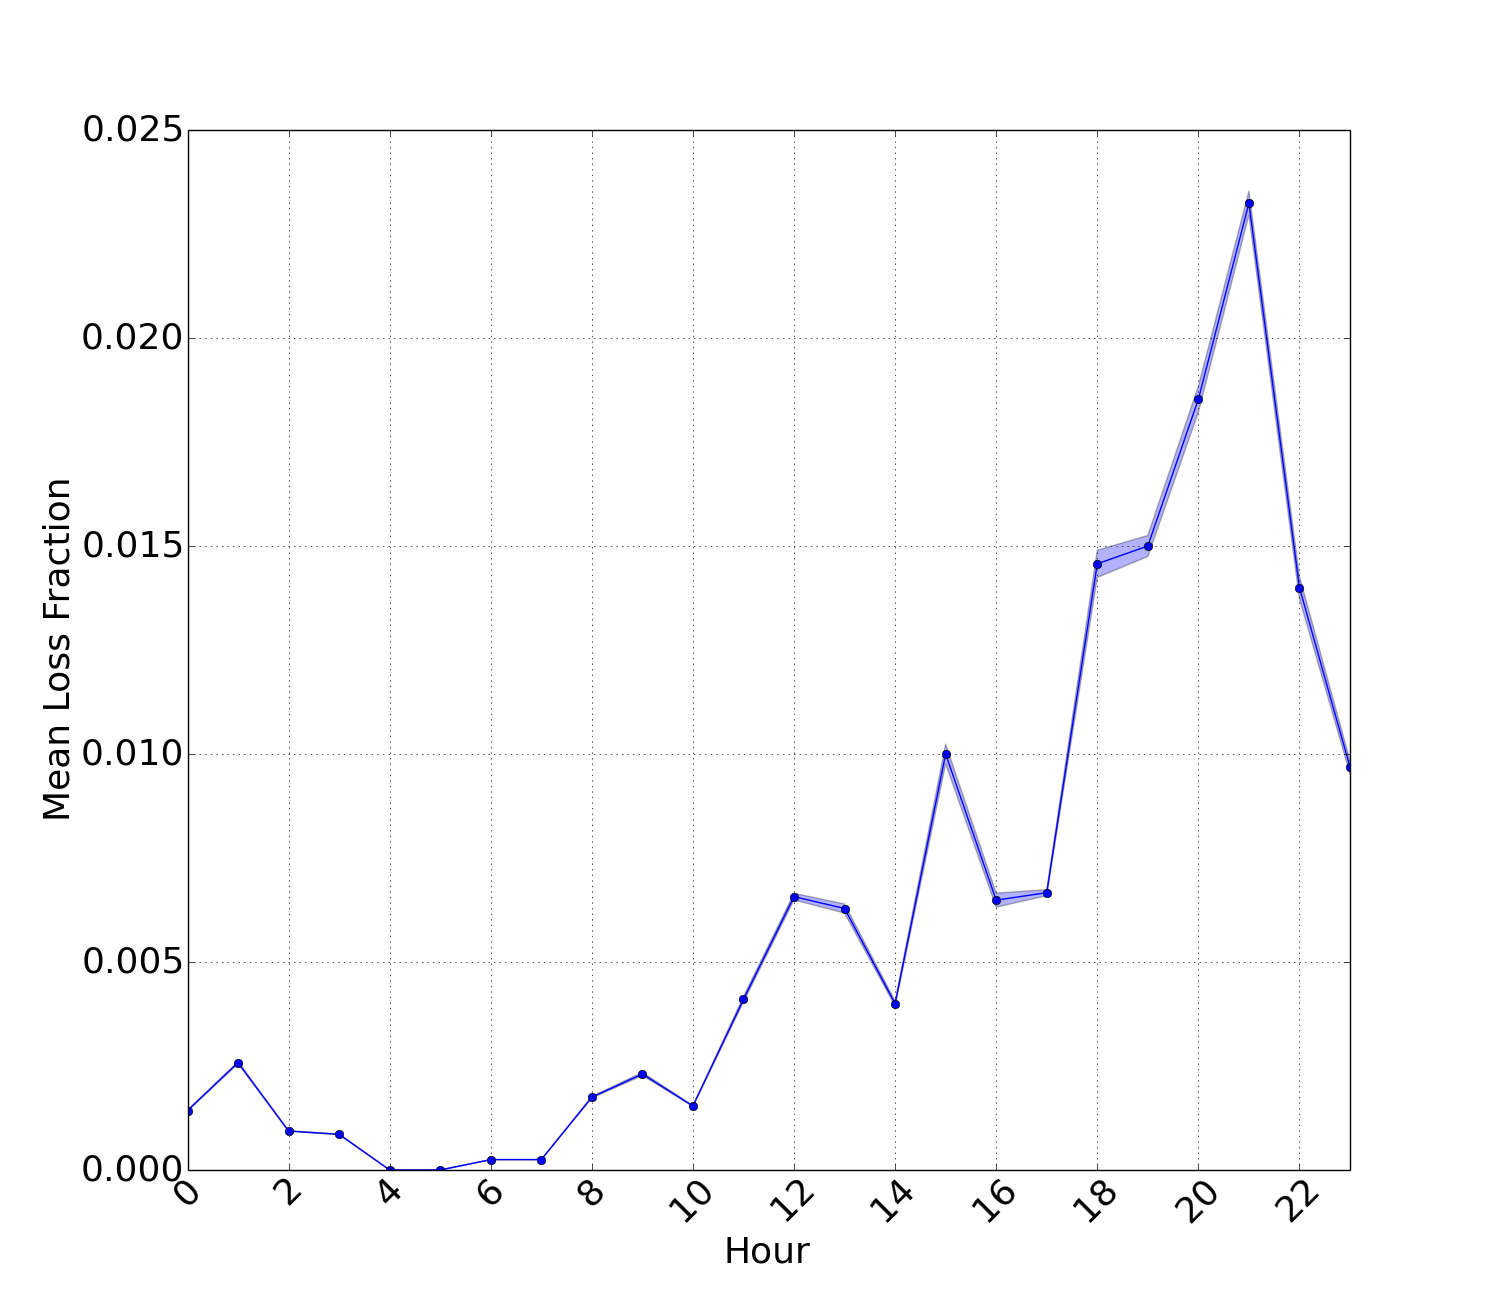
\includegraphics[width=1.0\textwidth]{./figures/mean_per_hour_in_a_day_NHODTCSRV04_64:66:B3:50:06:90.png}
        \caption{Mean and variance per hour}
    \end{subfigure}%
    ~ 
    \begin{subfigure}[b]{0.5\textwidth}
        \centering
        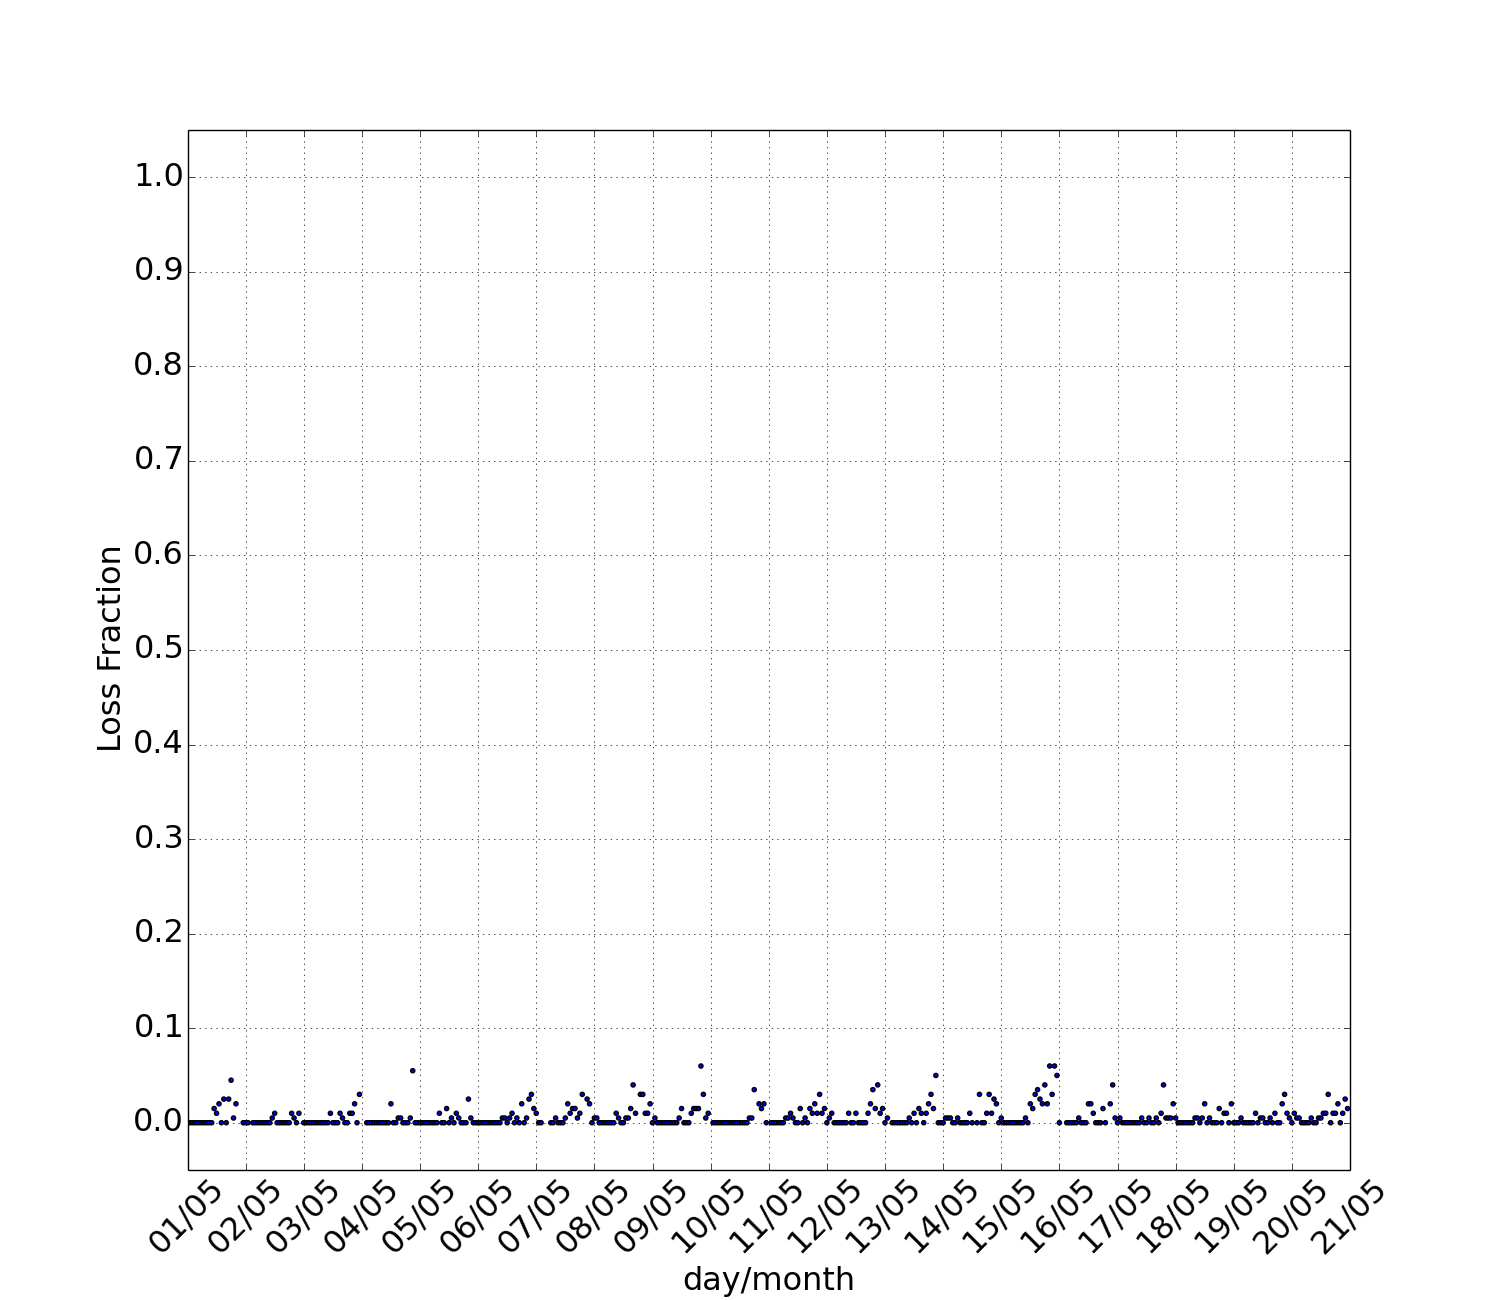
\includegraphics[width=1.0\textwidth]{./figures/ts_NHODTCSRV04_64:66:B3:50:06:90.png}
        \caption{Time Series}
    \end{subfigure}
    \caption{Client 1}
    \label{fig:mean_day_hour_ts}
\end{figure}

% - mean loss by week day of single client\\
% - power spectra to check periodicity? \\

\section{Change Points Dataset}

There are several approaches to construct a change points dataset to test a change point detection method. Some works in the literature simply create a simulated time series thorugh generative models, however different segments are generated by the same model but with different parameters. In general, this types of time series are more easily handled in change point detection algorithms, since some methods assumes the same models that generated the data or because real data can have more complex characteristics. Another way is to create a time series appending different segments provenient from different real time series data. In this cases is easy to simplify the dataset since some characteristics as the segments lengths are defined by the dataset creator and another ones are fakely introduced. Another works assumes that the latent information of the time series are available, and with specific knowledge of the application field, it is possible to assume what kinds of configuration changes could induce a change in the time series. In the case of the application field of the present work this would be difficult, since the latent information would be connected with the network situation such as network topology, characteristics of routers congestions, physical equipments problems, which is a too complex, or even impossible information to collect and also to assume which variables could impact the time series. Other apprach also uses the latent information but instead creates a controlled environment in which is possible to change the configuration over time, but as in the previous case, this would be too complex. The approach followed by this work was to use a visual annotation of the time series. It were conducted, with an application domain specialist, visuallyu indicating the relevant changes. It is known that human visual inspection methods can bring erroneous conclusions, but with the data and application scenarion it was the best fit, as network engineers visually identify, after simple automatic filters, the change points.

This work is interested in work directly with real data and satisfy a real application problem.

As in other tasks, it is difficult to translate a human visual perception in a sistematically method.

In general, when the exact types of target changes are previously know the problem is easier.

\section{Methodology}

\section{Descriptive Analysis}

- explain possible ways to get the ground truth\\
- description of the volunteer\\
- user instructions\\
- snapshots of system\\ 
- how time series were selected to be in the survey\\

\section{Description of Change Points Dataset}

- number of time series, number of change points: it is a high dimensional problem\\
- distribution number of changes per time series\\
- distribution time between change points\\
- distribution time for the first change point\\
- distribution time from last change point to time series end\\
- distribution of classification time?\\
- measure the difference between consecutive segments?\\

\section{Performance Evaluation}

- how the performance is asserted in literature\\
- ROC curve\\
- confusion matrix and accuracy metrics\\
